\appendix

\section{Appendices}
\label{sec:appendix}
\small

\subsection{BERT fine-tuning figures}

BERT$_{large}$ was fine-tuned for both span annotation and classification tasks; below are tables and blots indicating the performance for each task.

\begin{figure}[h]
	\centering
	\begin{subfigure}{0.95\textwidth}%
		\centering
		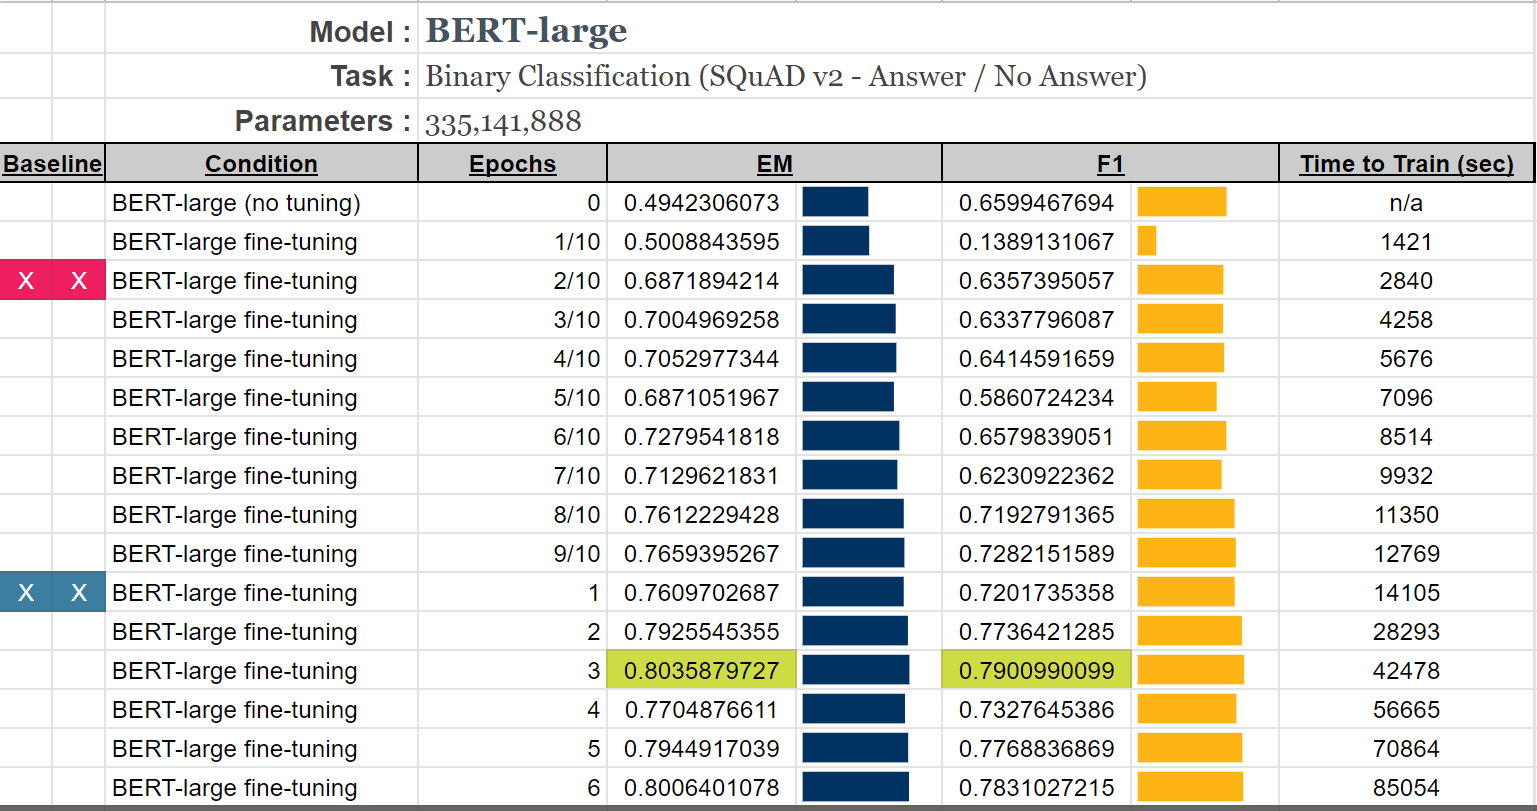
\includegraphics[width=\linewidth]{images/classification/BERT_Large_Training.png}%
		\caption{BERT$_{large}$ fine-tuning table : classification}
	\end{subfigure}%

	\vspace*{8pt}%
	
	\begin{subfigure}{0.96\textwidth}%
		\centering
		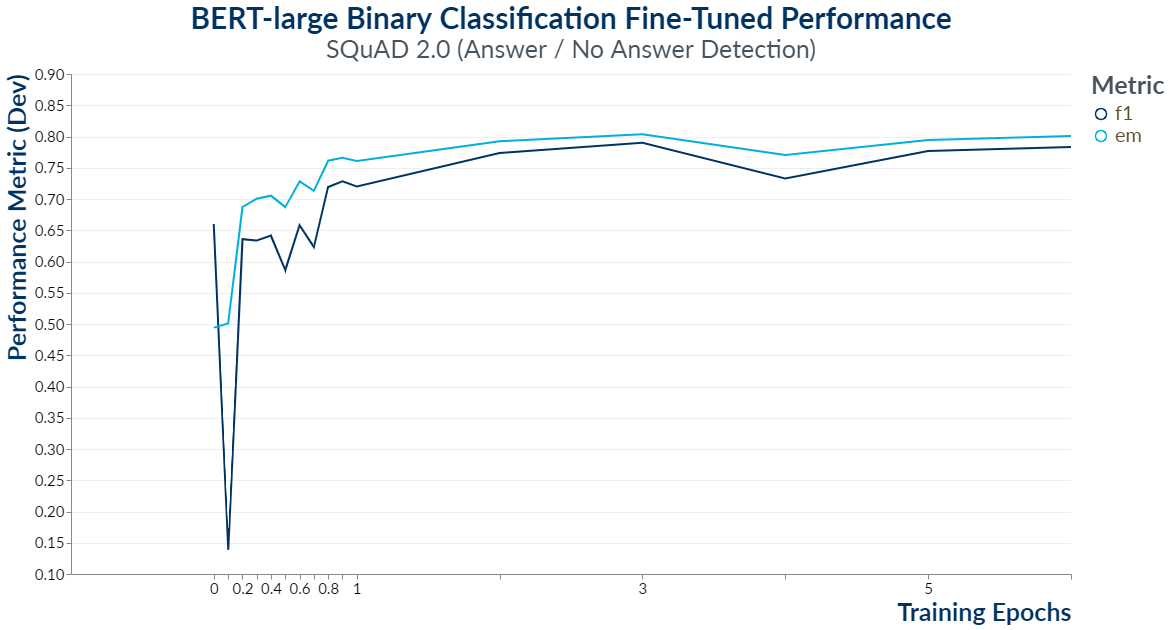
\includegraphics[width=\linewidth]{images/BinaryClassification_BERT_Training_Performance_plot.png}%
		\caption{BERT$_{large}$ fine-tuning plot : classification}
	\end{subfigure}%
	\caption{\label{apdx:BERT_fine_tuning_classification}BERT$_{large}$ fine-tuning for classification}
\end{figure}%

\begin{figure}[!h]
	\centering
	\begin{subfigure}{0.95\textwidth}%
		\centering
		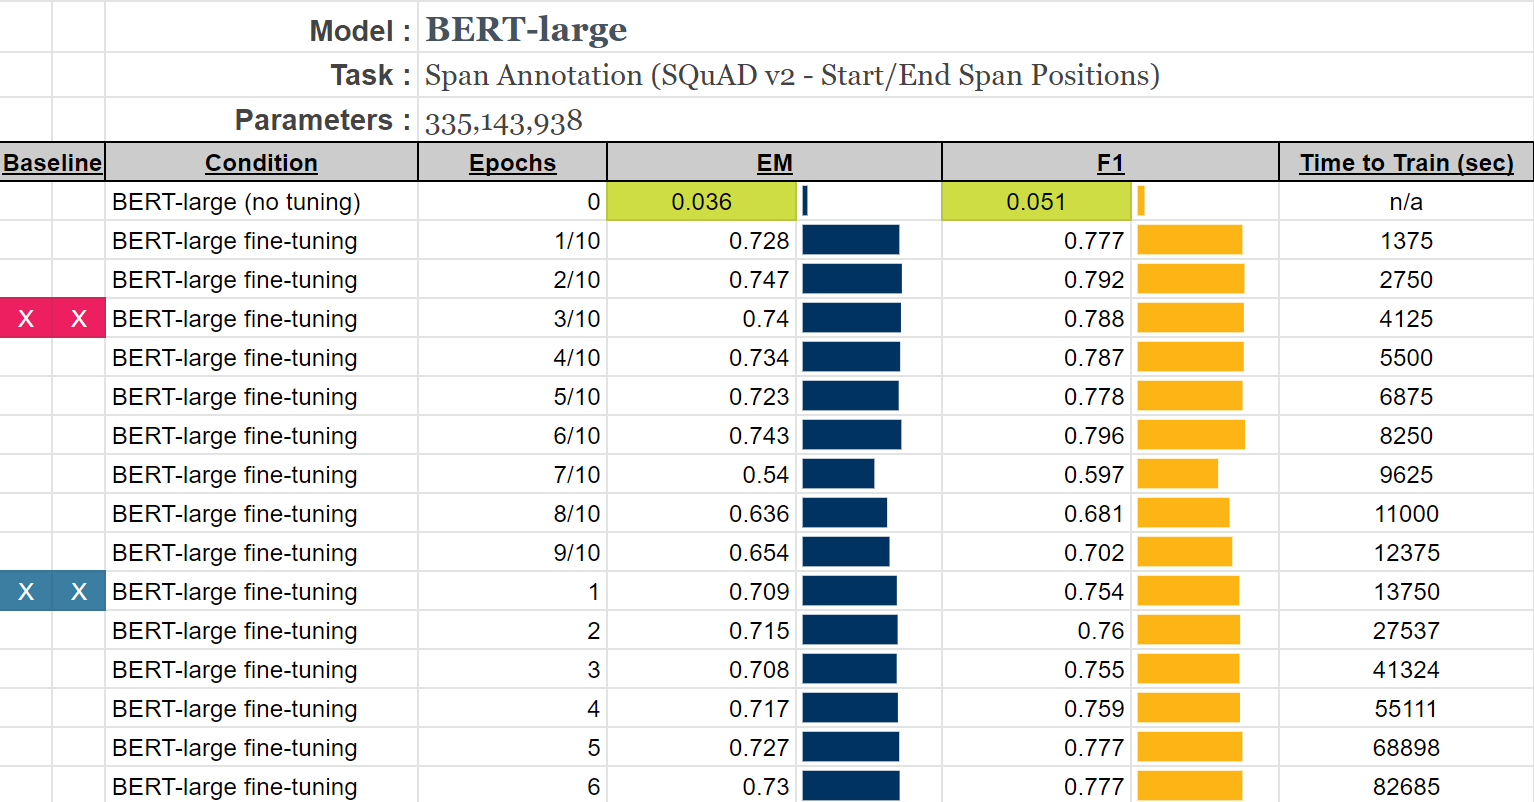
\includegraphics[width=\linewidth]{images/span/BERT_Large_Training.png}%
		\caption{BERT$_{large}$ fine-tuning table : span annotation}
	\end{subfigure}%
	
	\vspace*{8pt}%

	\begin{subfigure}{0.96\textwidth}%
		\centering
		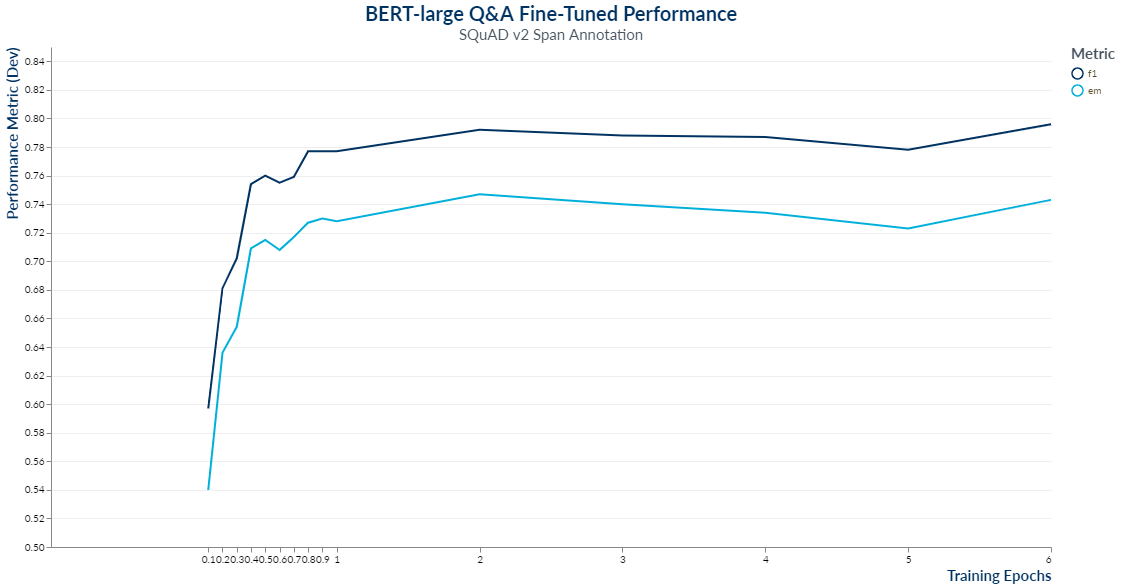
\includegraphics[width=\linewidth]{images/QnA_BERT_Training_Performance_plot.png}%
		\caption{BERT$_{large}$ fine-tuning plot : span annotation}
	\end{subfigure}%
	\caption{\label{apdx:BERT_fine_tuning_span_annotation}BERT$_{large}$ fine-tuning for span annotation}
\end{figure}

\newpage
\subsection{Table of all model results for span annotation}
\label{apdx:span_annotation_all_results}

Models were trained on embeddings derived from 3/10 of an epoch and 1 full epoch.  Performance on evaluation of the dev set is presented below.

\begin{figure}[h]
	\centering
	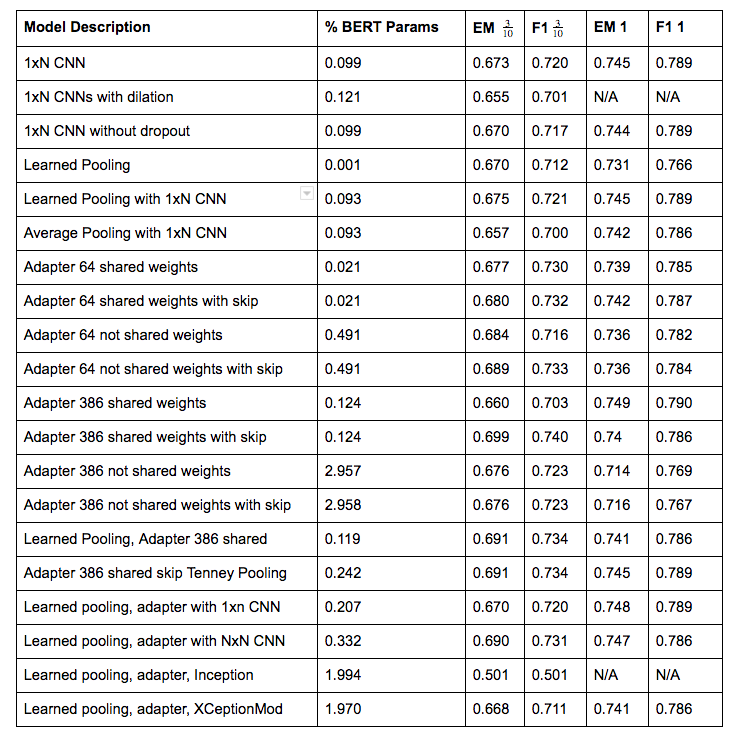
\includegraphics[width=\linewidth]{images/span/Span_Annotation_All_Model_Results.png}%
	\caption{BERT$_{large}$ All model performance : span annotation}
\end{figure}

\subsection{Best model performance for classification task}

The best model evaluated for the classification task was a simple linear model that performed channel contraction using learned weights followed by a simple dense layer connection with no softmax.  As indicated below, this model outperformed BERT$_{large}$ for almost every metric save for F1 on 3 epoch fine-tuned embeddings.

\begin{figure}[h]
	\centering
	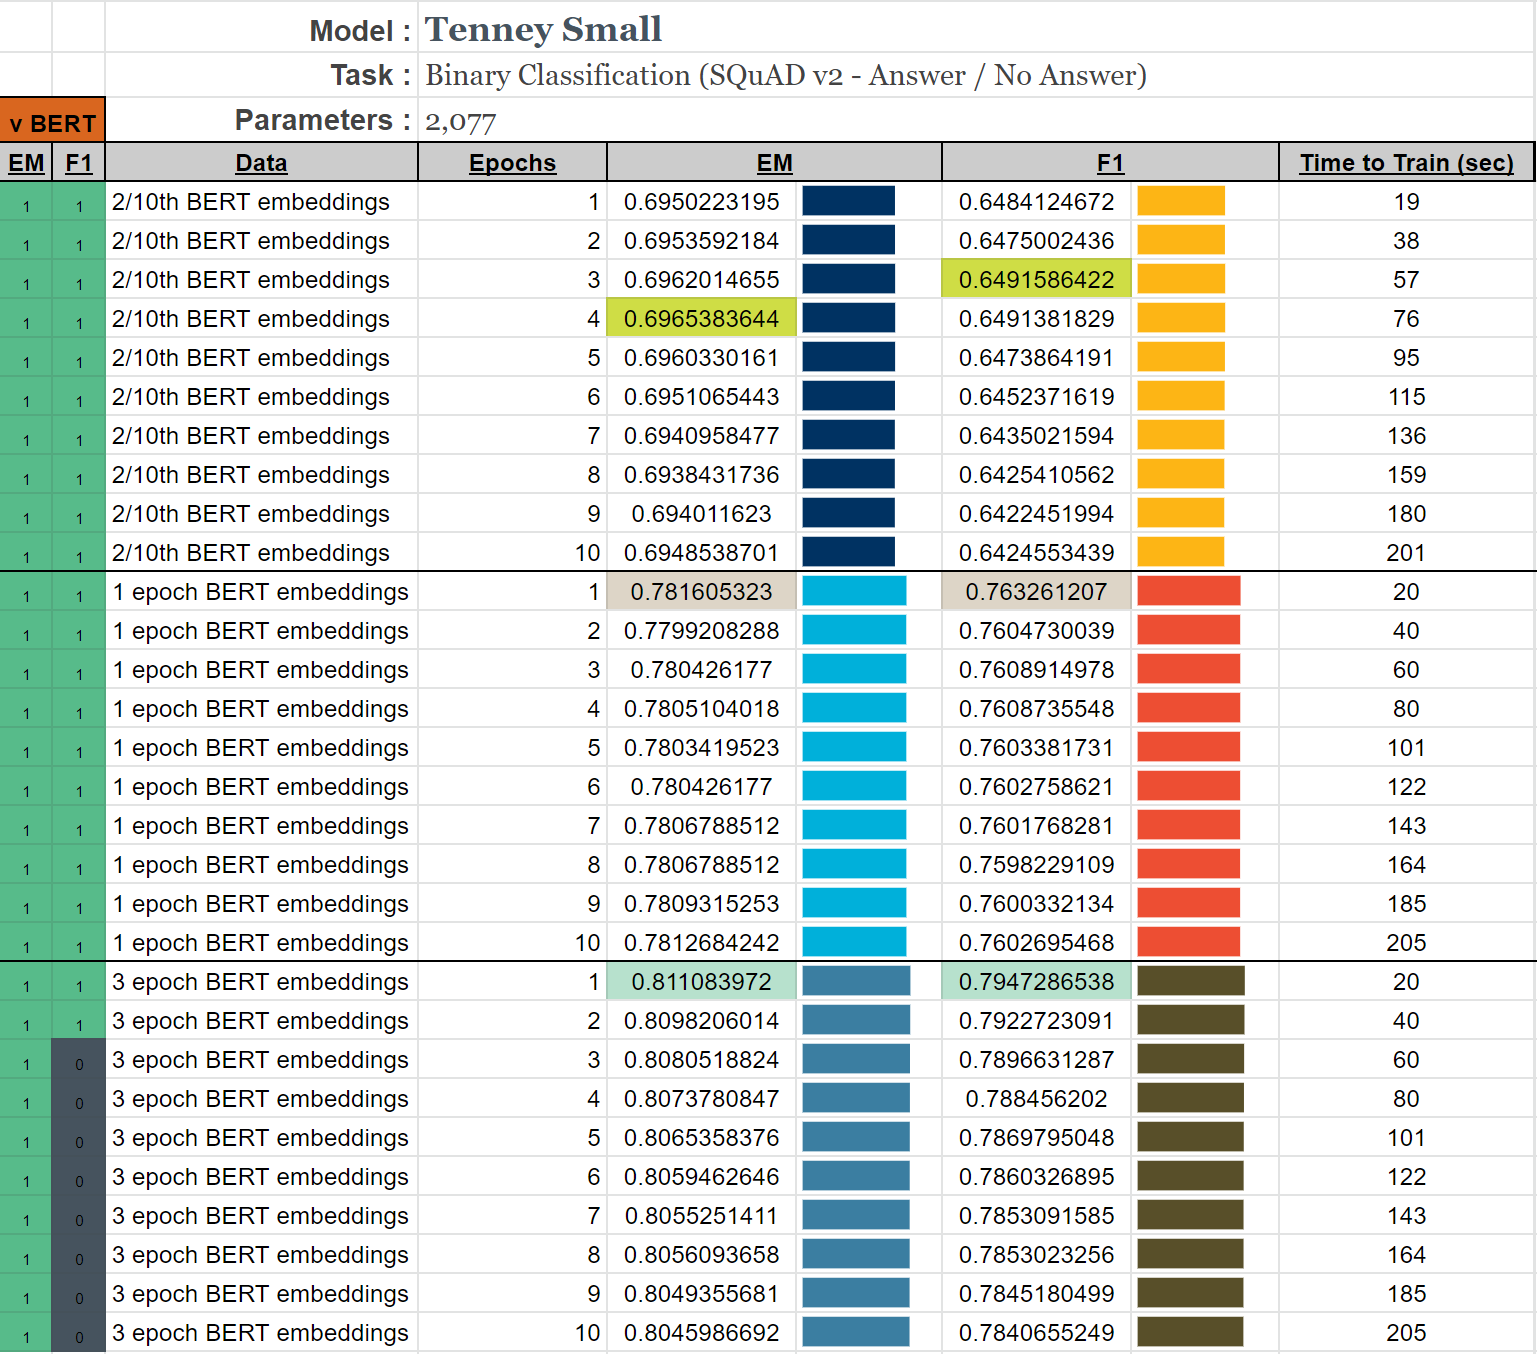
\includegraphics[width=\linewidth]{images/classification/TenneySmall_Training.png}%
	\caption{BERT$_{large}$ Best model performance : classification task}
\end{figure}

\newpage

\begin{figure*}[t]
	\centering
	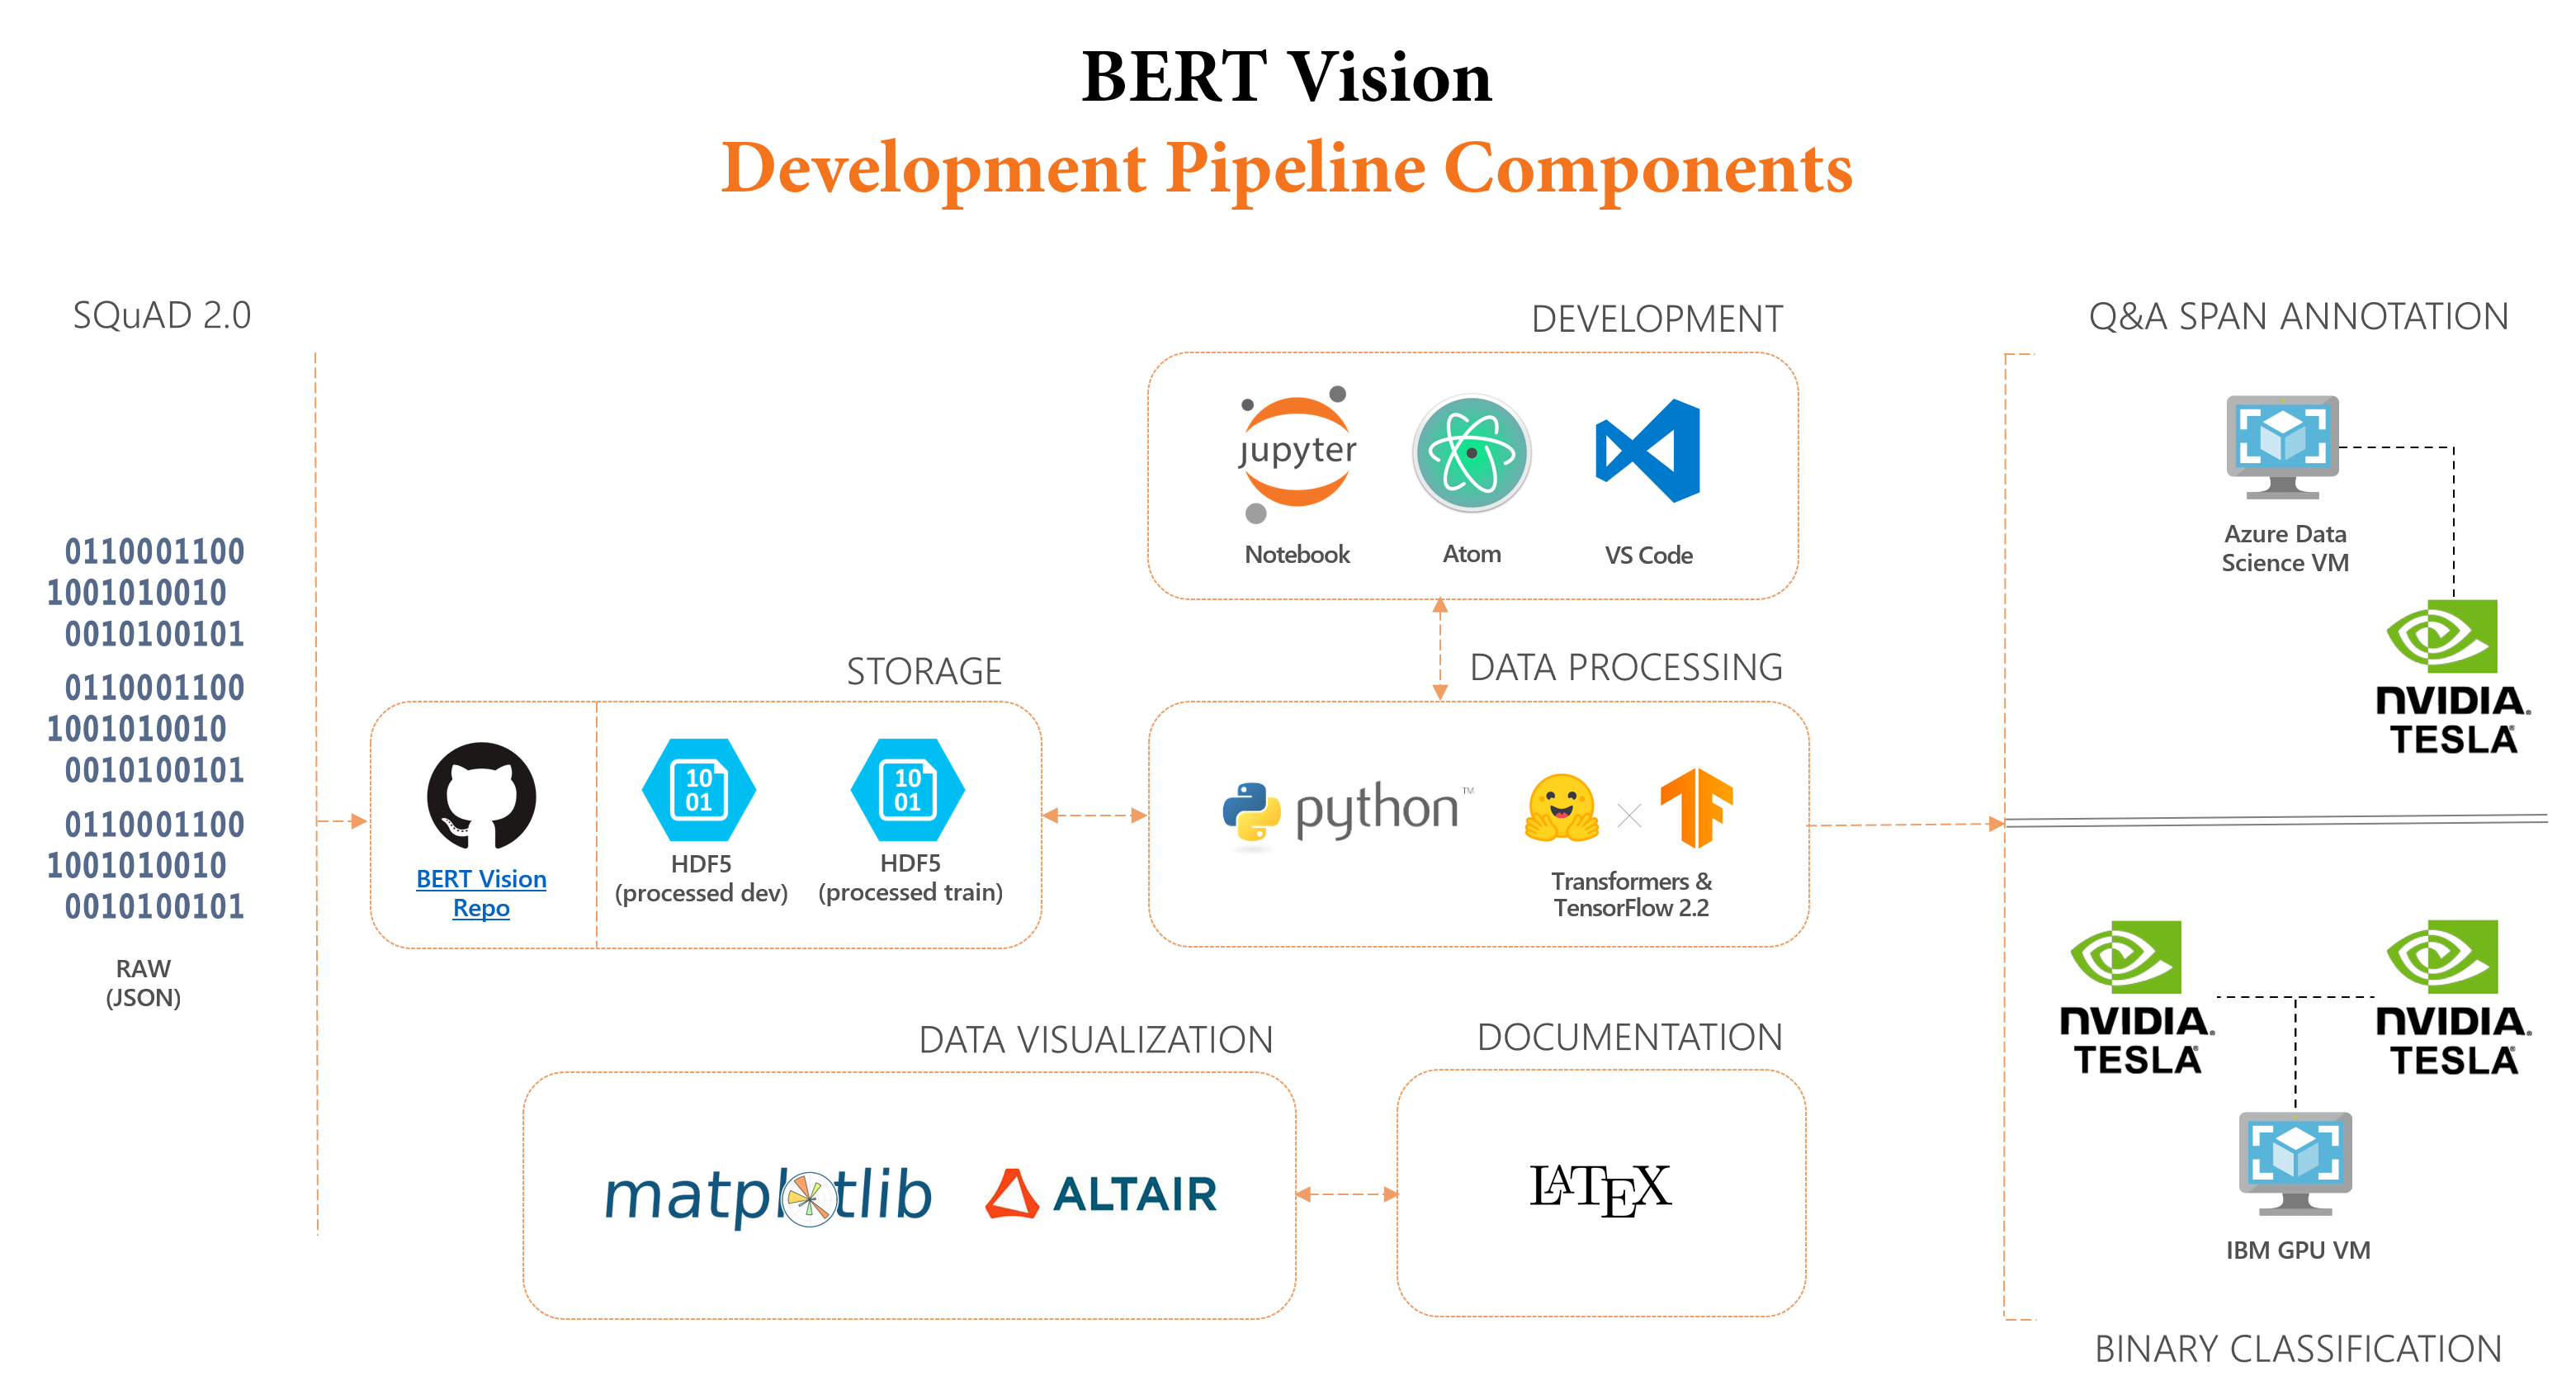
\includegraphics[width=\textwidth]{images/BERTVision_Development_PIpeline.png}%
	\caption{BERTVision development pipeline}
	\label{apdx:bertvision_development_pipeline_graph}
\end{figure*}

\newpage

\subsection{Table of all model results for classification}
\label{apdx:classification_models_trained}

Models were trained on BERT$_{large}$ fine-tuned embeddings derived from 2/10 of an epoch and 1 full epoch. Additionally, the most successful model was trained on 3 epochs fine-tuned embeddings. Performance on evaluation of the dev set is presented below.

\begin{table}[h]
	\centering
	\small
	\begin{tabular}{L{2.9cm}|C{1.5cm} C{0.9cm} C{0.9cm}}
		\toprule
		\textbf{Model} & \textbf{\% Params} & \multicolumn{2}{c}{\textbf{SQuAD2.0}}\\
		& \textbf{BERT}$_{large}$ & \textbf{EM} & \textbf{F1}\\
		\midrule
		adapter pooler tenney 	& 0.119\% & 0.685 & 0.646 \\
		xception abbr 			& 0.079\% & 0.673 & 0.702 \\
		\textbf{xception}		& \textbf{6.181\%} & \textbf{0.707} & \textbf{0.710} \\
		xception abbr cls 		& 0.080\% & 0.672 & 0.564 \\
		adapter pooler avg 		& 0.119\% & 0.691 & 0.624 \\
		tenney small 			& 0.001\% & 0.697 & 0.650 \\
		\bottomrule
	\end{tabular}
	\caption{Models trained on embeddings at $\frac{2}{10}e$}
\end{table}

\begin{table}[h]
	\centering
	\small
	\begin{tabular}{L{2.9cm}|C{1.5cm} C{0.9cm} C{0.9cm}}
		\toprule
		\textbf{Model} & \textbf{\% Params} & \multicolumn{2}{c}{\textbf{SQuAD2.0}}\\
		& \textbf{BERT}$_{large}$ & \textbf{EM} & \textbf{F1}\\
		\midrule
		adapter pooler tenney 	& 0.119\% & 0.781 & 0.765 \\
		\textbf{xception abbr}	& \textbf{0.079\%} & \textbf{0.785} & \textbf{0.782} \\
		xception 				& 6.181\% & 0.783 & 0.766 \\
		xception abbr cls 		& 0.080\% & 0.783 & 0.780 \\
		adapter pooler avg 		& 0.119\% & 0.779 & 0.765 \\
		tenney small 			& 0.001\% & 0.782 & 0.763 \\
		\bottomrule
	\end{tabular}
	\caption{Models trained on embeddings at $1e$}
\end{table}

\begin{table}[h]
	\centering
	\small
	\begin{tabular}{L{2.9cm}|C{1.5cm} C{0.9cm} C{0.9cm}}
		\toprule
		\textbf{Model} & \textbf{\% Params} & \multicolumn{2}{c}{\textbf{SQuAD2.0}}\\
		& \textbf{BERT}$_{large}$ & \textbf{EM} & \textbf{F1}\\
		\midrule
		tenney small & 0.001\% & 0.811 & 0.795 \\
		\bottomrule
	\end{tabular}
	\caption{Models trained on embeddings at $3e$}
\end{table}

\subsection{Data challenges and training time}
\label{apdx:data_challenges}

During training, in order to obtain the internal BERT embeddings for each example (which is the input “data” into our downstream models), we had to either: 1.  Pre-generate the embeddings, or 2. Generate the embeddings for each example on the fly from a frozen BERT model. Due to the size of BERT, we quickly ran out of GPU memory with the second method, so we had to resort to the first. Working with BERT embeddings on the SQuAD 2.0 data set presented a data engineering problem due to the size of the data. Using the 4-byte float representation, the entire dataset with each example having shape (386, 1024, 25) is approximately 5 TB in size, which is far too large to store into memory on our hardware. Instead, this data was written to disk, and a custom Keras data generator used to retrieve this data in batch sizes of 16 for training (in a shuffled random order).

While this method presents no cost to accuracy, the I/O time for loading the data was significant, much longer in most cases than the actual training time for fitting any of our models. For all models, training per epoch was around 5 hours, but we estimate that on average over 95\% of the time is spent on loading data, and only 5\% of the time fitting the model. As a result, in this work, in order to separate out infrastructure issues with model training, as a proxy for training cost, we compare the number of parameters in our model rather than wall clock training time. We also explore the potential to use less embedding data during fitting, and for future work, a faster storage system should be explored in order to advance this work for practical applications. 

We also note that for the classification task, we did not experience any data management issues. Since we only use the CLS token for classification rather than the entire sequence length of 386, the full embeddings of all examples were a little over 13GB, which easily fit into CPU memory. Training for each epoch for on the order of minutes rather than hours.

\subsection{Model training strategy}
\label{apdx:model_training_strategy}

We train all of these models for a single epoch for three reasons: 1. Performance was already desirable at a single epoch. 2. Further training typically did not help performance further, 3. Due to our data management issue, loading the data usually takes more than 95\% of the training time, which makes it difficult to train for extended numbers of epochs (See [\ref{apdx:data_challenges}]). 

\subsection{Explanation on the shape of input embeddings data}
\label{apdx:explanation_of_input_embeddings_shape}

For span annotation, for a single SQuAD 2.0 example, the data point has a shape of (386,1024,25). Here, 386 represents the text length dimension, and 1024 the BERT embedding dimension for each encoder layer. The 25 comes from the stacking of the contextual wordpiece \cite{DBLP:journals/corr/WuSCLNMKCGMKSJL16} text embeddings, the 23 hidden state activations, and the final sequence outputs (24th layer) for BERT. 

For classification, an example has input shape (1,1024, 26). Here, 1 represents the lone CLS token, 1024 the BERT embedding dimension. The 26 comes from the stacking of the contextual wordpiece text embeddings, 23 hidden state activations, the final CLS token for the output encoder layer (24th layer), and the pooled CLS token from the final pooler layer.

\subsection{Explanation on max sequence length input into BERT}
\label{apdx:explanation_max_sequence_length}

BERT$_{large}$ has a maximum input sequence length of 512. While we could have truncated our question-context pairs at this length, we found that a large majority of examples were much shorter than this length. The average length of the input is about 171 tokens long. The length we chose was 386, which is between 98-99th percentile. As a result, without much loss, we can significantly save on the number of mostly meaningless “[PAD]” tokens we needed to store, especially for full 25-layers of BERT embeddings.

\subsection{CNN models preserving max sequence length}
\label{apdx:cnn_models_preserving_seq_length}

Our CNN models were all designed to preserve the sequence length of the input question-context pair. This was achieved with 1xN convolutions so that these filters only compress along the 1024 dimension, or with NxN convolutions with padding along the sequence token dimension. In the case of 1xN convolutions, this is similar to a unigram model that treats each token separately. The NxN convolutions were n-gram models, ranging from 1 - 7 (depending on the size of N). The reason we did this is because we also tried convolution blocks from Inception [1] that gradually shrinks the 386 dimension; however, this model failed to learn to even fit the training data. As a result, we believe that for span annotation, since the data starts with a 386 dimension representing token position, and ends by predicting a probability for each position, we need this sentence length dimension throughout the entire model. A traditional computer vision CNN model such as Inception shrinks the image along this dimension, which destroys the structure necessary for span detection. Shrinking the text length and later expanding it again loses information, resulting in a failure to fit the data.

\subsection{Comparison of our BERT performance with Devlin}
\label{apdx:comparison_with_devlin}

For our fine-tuning procedure, we observed that performance peaked at 2 epochs, achieving an Exact Match (EM) of 0.747, and an F1 score of 0.792. This is slightly worse than that reported by \cite{Devlin2019} at an EM of 78.7 and F1 of 81.9. We hypothesize that these difference might arise due to our training batch size, random initializations, and the fact we do not favor the null answer by a "$\theta$" threshold, where "$\theta$" was optimized based on dev set performance (see Section 4.3 in Devlin). We use purely the softmax probabilities output by the model without favoring no answer by an optimized threshold based on the dev set itself.

\subsection{Where to exact embeddings}
\label{apdx:where_to_extract_embeddings}

We wished to extract embeddings at two stages in the training process: 1. Early-on so that BERT fine-tuning is cheap, and the embeddings are amenable to use as data for modeling, 2. At a slightly later stage before convergence so that our models have a chance to achieve or outcompete the best performing BERT model. 

For span detection, our learning curve for full-epoch BERT fine-tuning shows that 1 epoch is relatively decent compared to peak performance at 2 epochs, which gives us a chance to outperform our best observed BERT performance (goal 2). At the same time, fine-tuning for a full epoch on all of SQuAD 2.0 takes around 5 hours, which is already very expensive. To this end, we explored BERT performance every 1/10 of a fractional epoch between 0 and 1. We see that both EM and F1 are increasing steadily in our single run, with a large jump between fractional epochs 3 and 4. In addition to 1 epoch, we extracted embeddings at 3/10 of an epoch immediately before this jump, which took approximately 1.5 hours of fine-tuning. We believe this is a decent spot because such partial fine-tuning is relatively cheap, and performance has yet to jump, giving us an opportunity to improve performance using our models (goal 1).

For classification, looking at our learning curve for full-epoch fine-tuning, 1 epoch is yet again a clear candidate for extracting the embeddings (goal 2). Performance is already relatively decent compared to peak performance at 3 epochs, but takes $\frac{1}{3}$ time and compute resources to train. For goal 1, we extracted embeddings at 2/10 of a fractional epoch between 0 and 1. We see a clear jump in performance between 1/10 of a fractional epoch and 2/10, a jump we do not observe again until 8/10. Therefore, from the dev set perspective, 2/10 is a high value fractional epoch, whether 3/10 - 7/10 does not add much to the performance of the model.

\subsection{Need to fine-tune}
\label{adpx:need_to_fine_tune}

Using a variety of parameter-efficient CNNs and dense architectures, we found such models were unable to fit BERT hidden state activations without fine-tuning to our specific QA task SQuAD 2.0. This discovery is consistent with the observations made in \cite{ma2019universal}, where the authors found that fine-tuned BERT on either SNLI and in-domain text corpus consistently outperformed pre-trained BERT without fine-tuning by a large margin for various tasks, including QA (although not on SQuAD). As a result, we decided mild amounts of fine-tuning was necessary in order to generate usable embeddings.

\subsection{Training hardware and development pipeline}
\label{apdx:training_hardware}

All span annotation training and inferencing was performed on a Microsoft Azure data science virtual machine with 112GiB onboard ram and a single NVIDIA Tesla TITAN series V100 Tensor Core GPU capable of ~7 TFLOPS double-precision and tensor performance of ~112 TFLOPS and possessed 16 GiB onboard RAM.  All binary classification training and experimentation was performed on an IBM virtual machine equipped with two NVIDIA Tesla TITAN series V100 Tensor Core GPU's (see [\ref{apdx:bertvision_development_pipeline_graph}]).

\begin{figure*}[t]
	\centering
	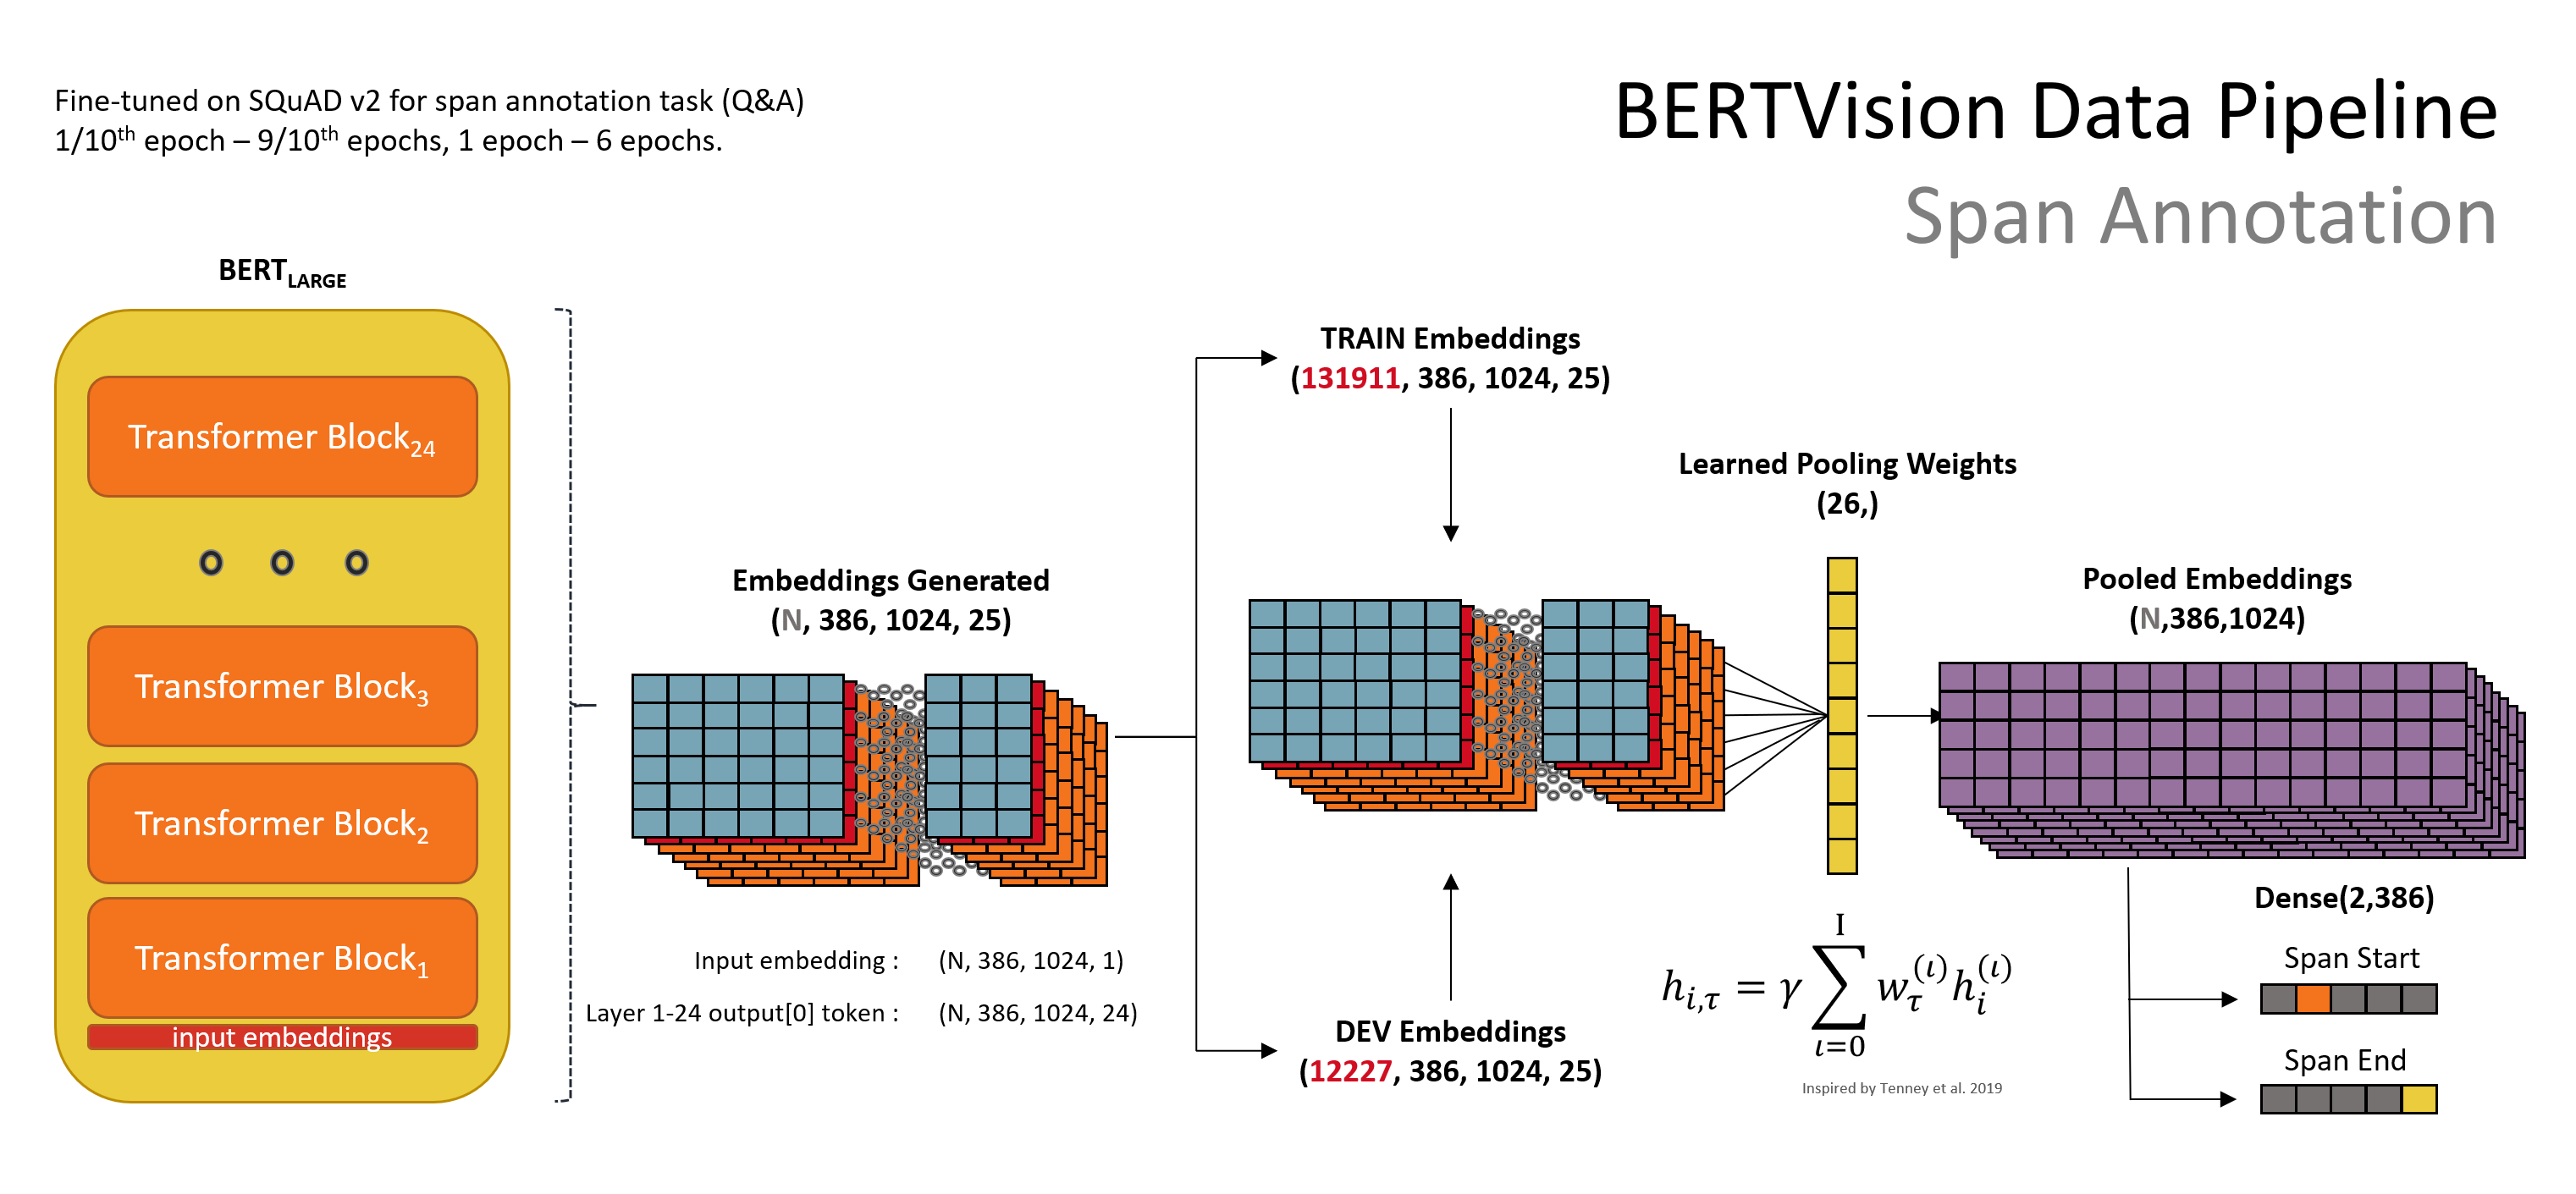
\includegraphics[width=\textwidth]{images/Data_Pipeline_Span_Annotation.png}%
	\caption{BERTVision span annotation data pipeline}
	\label{apdx:bertvision_span_annotation_data_pipeline_graph}
\end{figure*}

\begin{figure*}[!h]
	\centering
	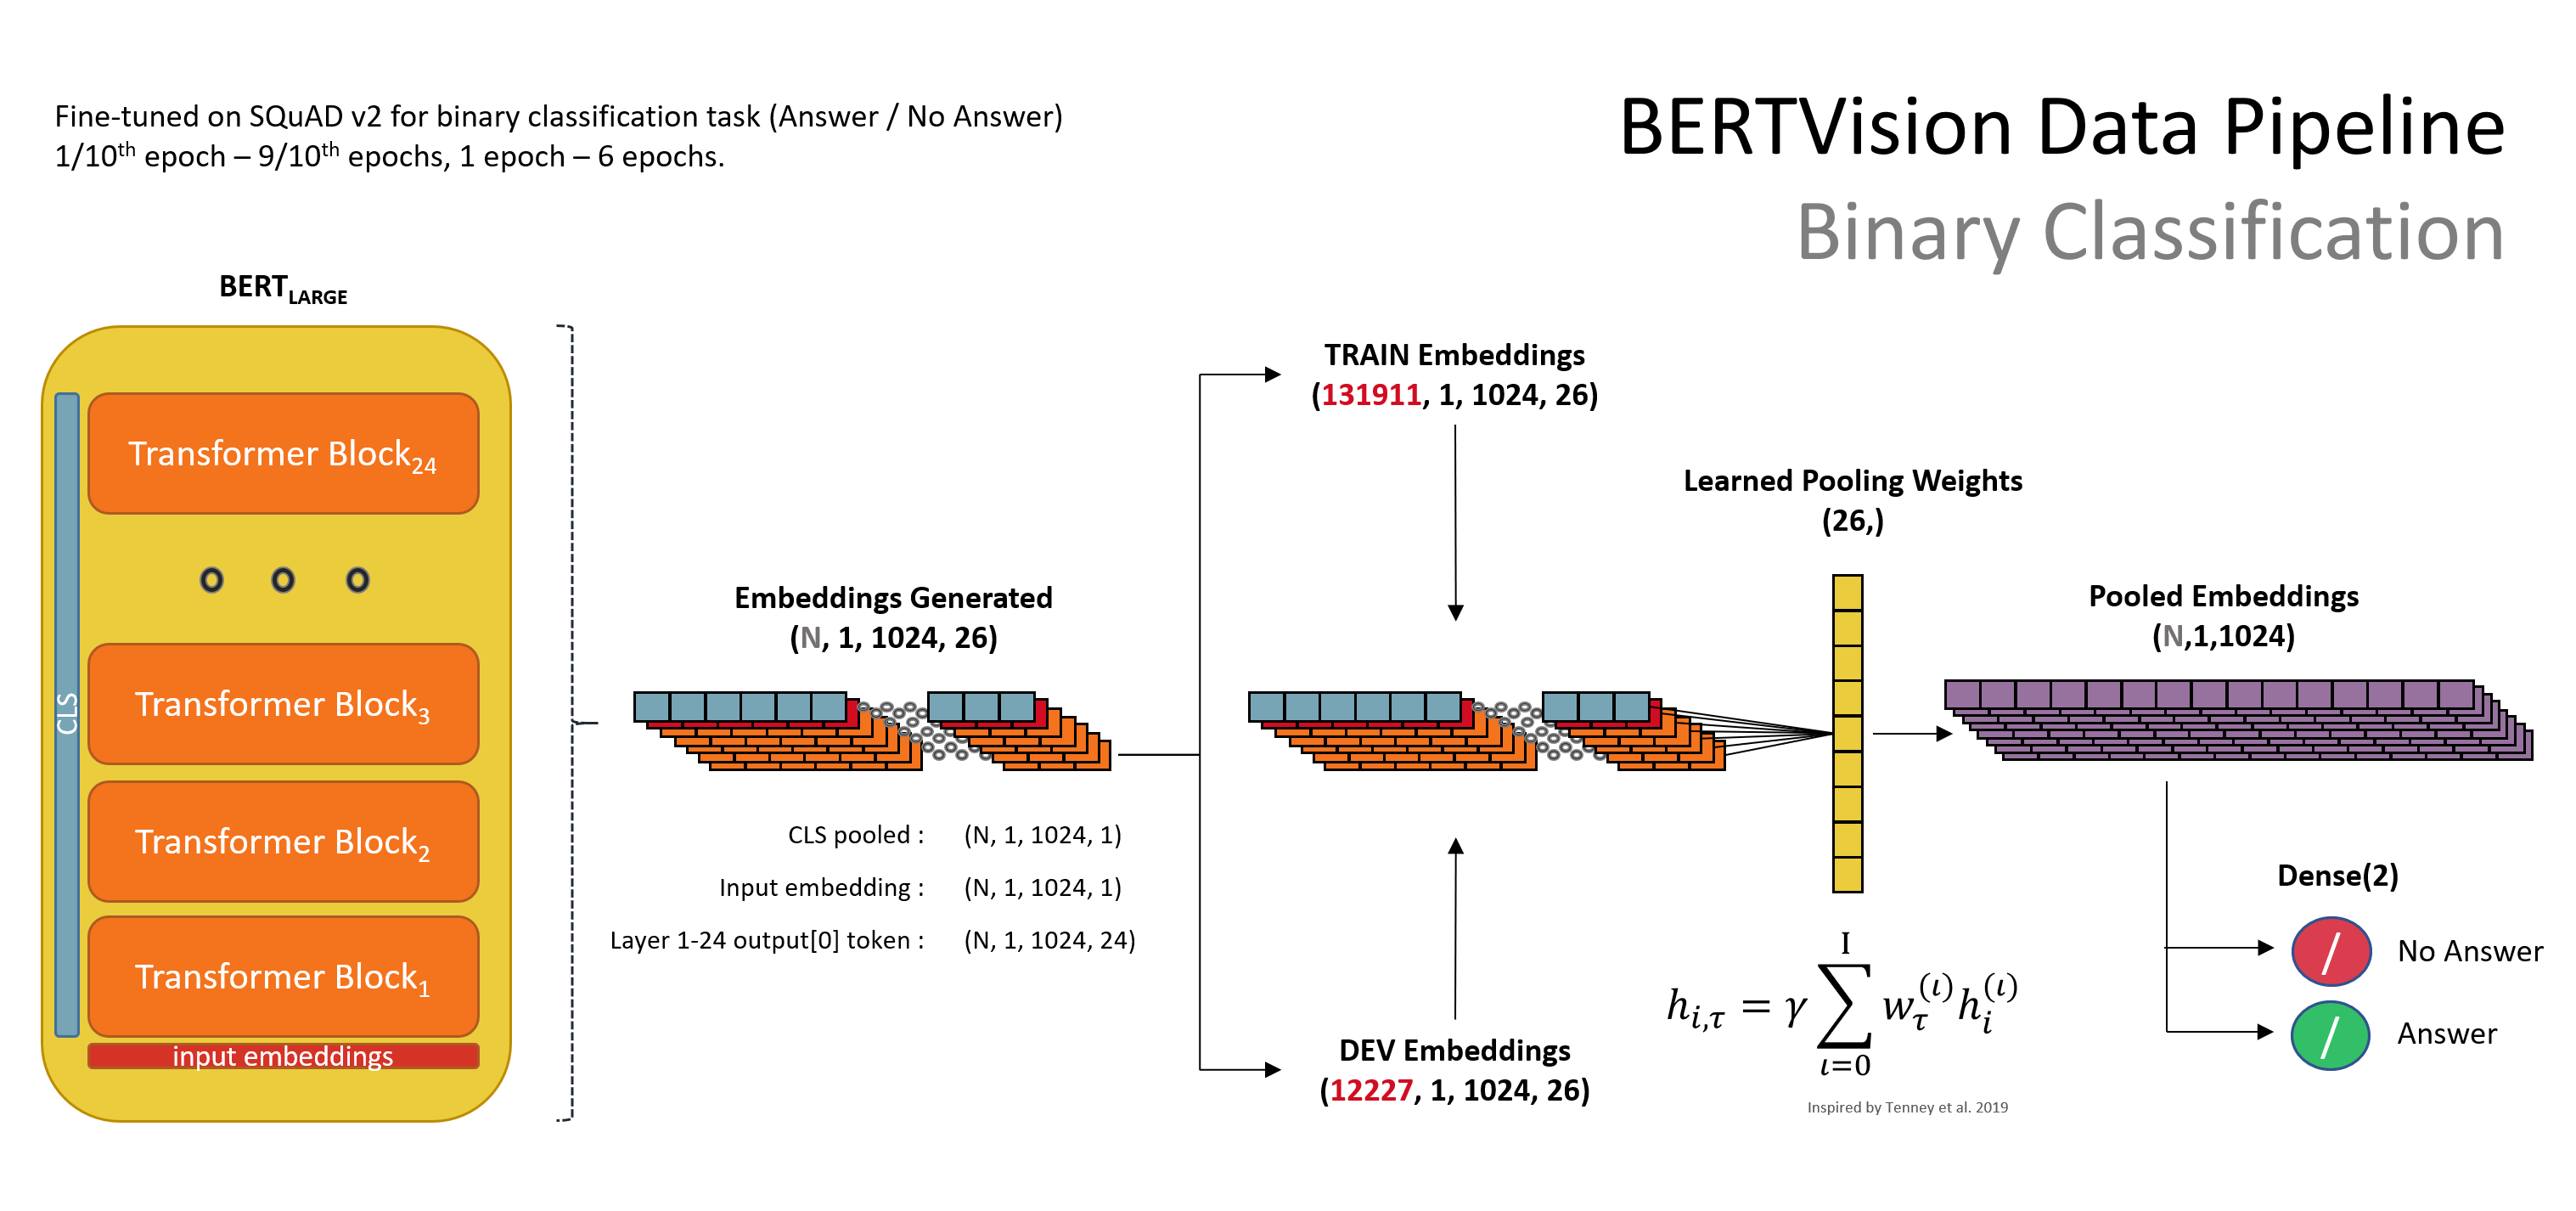
\includegraphics[width=\textwidth]{images/Data_Pipeline_Binary_Classification.png}%
	\caption{BERTVision classification data pipeline}
	\label{apdx:bertvision_classification_data_pipeline_graph}
\end{figure*}

\newpage

\subsection{Non-uniform weights}

Learned weights for learning pooling using the approach described in \cite{tenney-etal-2019-bert}. The model favors using later layers especially after layer 17. This is consistent with the observation in \cite{van_Aken_2019} that the last layers of BERT-base are much more accurate at supporting fact identification (which is the author’s proxy for span identification).

